\chapter{Completed Task}
\section{Word Embedding Visualization}
Word embeddings vectors were created using gensim word2vec model. Then the obtained 300 dimensional word embeddings vectors were converted into 2-dimensional and 3-dimensional vectors using Principal Component Analysis (PCA). The result obtained using the first 50 vectors were as follow:

\begin{figure}[H]
	\centering
	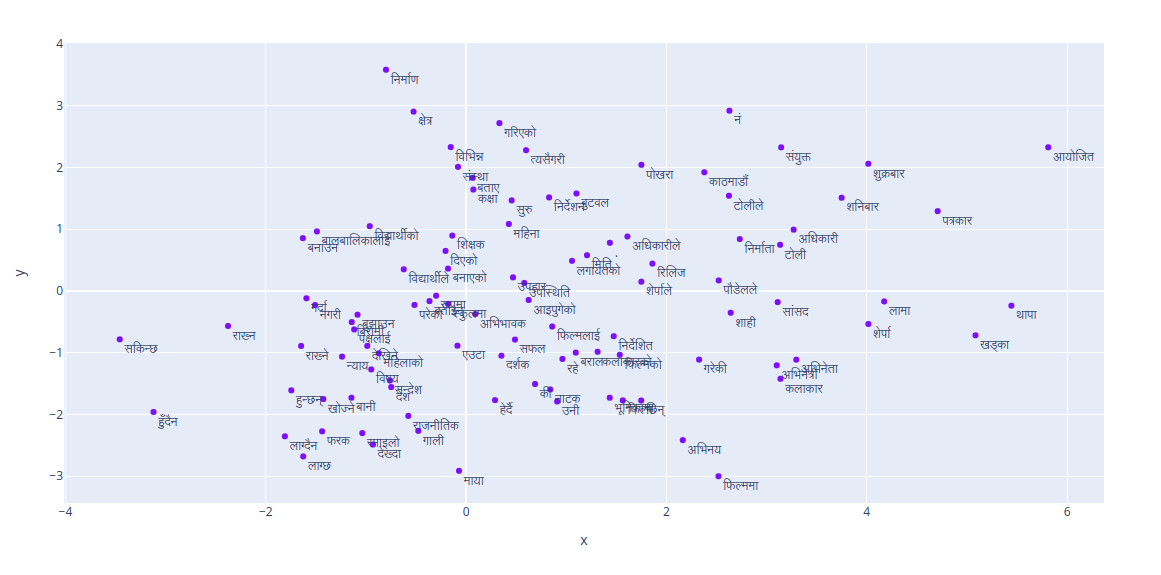
\includegraphics[scale = 0.4]{completed_task/2d.png}
	\caption{2d plot of word embeddings vectors}
	\label{fig:2d plot of word embeddings vectors}
\end{figure}

\begin{figure}[H]
	\centering
	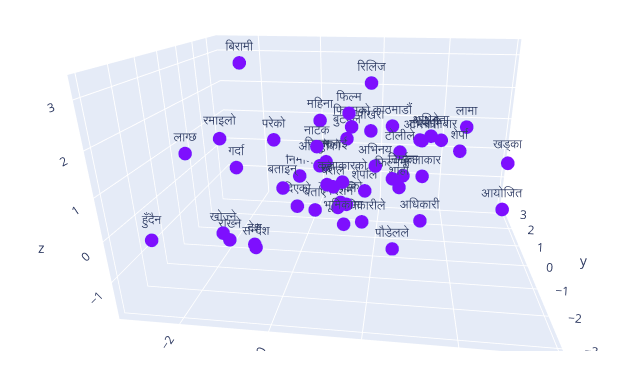
\includegraphics[scale = 0.5]{completed_task/3d.png}
	\caption{3d plot of word embeddings vectors}
	\label{fig:3d plot of word embeddings vectors}
\end{figure}


\section{Probabilistic Language Model}
For the development of a probabilistic language model, at first vocabulary was created from the training dataset. At first, the corpus was split into a list of sentences. Text preprocessing involves:

\begin{enumerate}
    \item remove all non-devanagari letters
    \item remove numbers from the corpus
\end{enumerate}


Then word tokenization was created which was used to create vocabulary from the tokenized word using the constraints of minimum frequency. Then, the n-gram count list was generated in which the count of various n-grams were stored. For the creation of our moder, unigram, bigram, trigram, 4-gram and 5-gram were created. Among these, the unigram, bigram and trigram performed better. 

Hence, we used only unigram, bigram and trigram for the probability estimation of the next word.

\begin{figure}[H]
	\centering
	\includegraphics[scale = 0.3]{completed_task/probabilistic_lm.png}
	\caption{Next word prediction using Probabilistic LM}
	\label{fig:Next word prediction using Probabilistic LM}
\end{figure}

\section{Transformer based language model}
For this language model too, the vocabulary was created using the same method as in the Probabilistic language model. Then the transformer architecture with 4 multi-head attention and 4 encoder layers were developed for language model training. Cross Entropy loss was used as a loss function and SGD was used as an optimizing function. The perplexity obtained is 568.5.

Input to the LM is current words and  num\textunderscore words to be predicted. Then the language model generate probable num\textunderscore words as shown in fig: \ref{fig:Next word prediction using Transformer based LM}

\begin{figure}[H]
	\centering
	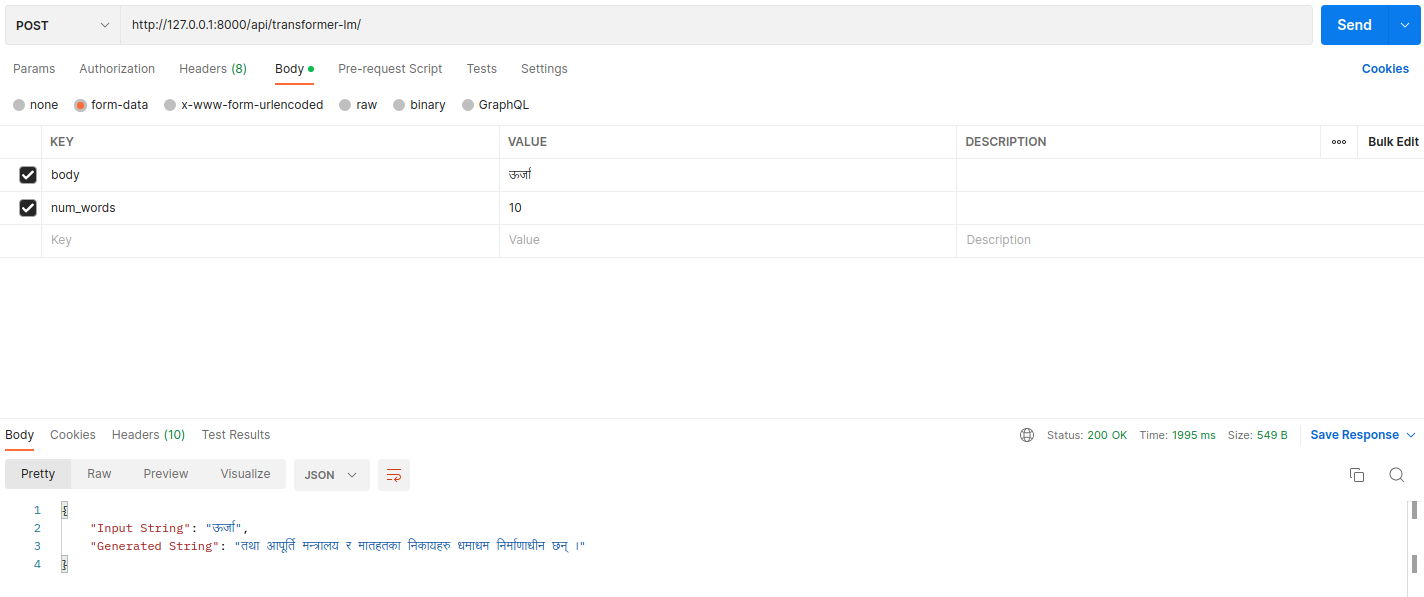
\includegraphics[scale = 0.3]{completed_task/transformer_lm.png}
	\caption{Next word prediction using Transformer based LM}
	\label{fig:Next word prediction using Transformer based LM}
\end{figure}

\section{Backend}
We have developed backend using Django and Django Rest Framework. For the API testing, Postman was used. Till today, backend for word embedding vectors, sentimental classification, probabilistic LM, transformer LM are completed.

\section{Frontend}
We have done the frontened for word embeddings,sentiment analysis(know the sentiment) and next probabable words upto now. The remaining part of the frontend will be done after the completion of remaining backend parts. You can see some of the frontend screenshots below to see the progress upto now. We will also be adding another mode as light mode for all these sections with the motive of providing more options for end user and for better user experience.


\begin{figure}[H]
	\centering
	\includegraphics[scale = 0.2]{completed_task/frontend/probabilistic_lm.png}
	\caption{Probabilistic language model frontend}
	\label{fig:Probabilistic language model frontend}
\end{figure}

\begin{figure}[H]
	\centering
	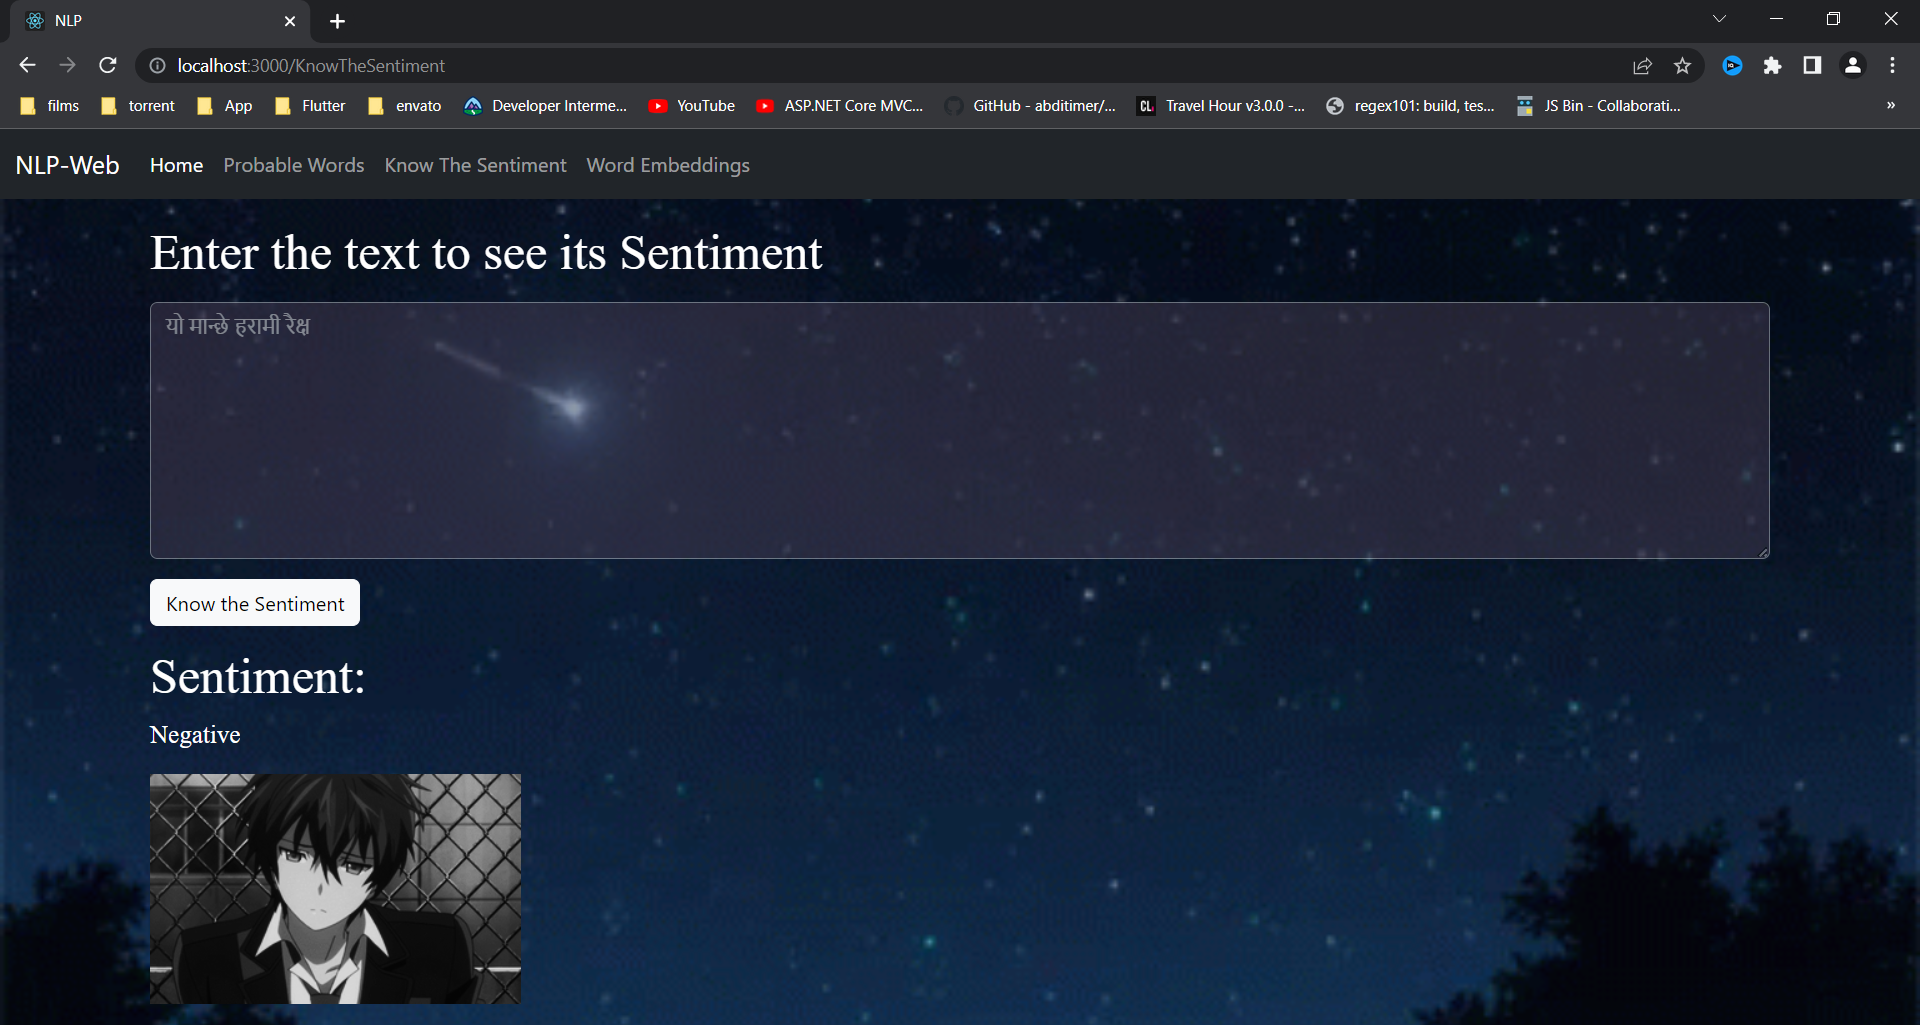
\includegraphics[scale = 0.2]{completed_task/frontend/sentiment.png}
	\caption{Sentiment classification (negative) frontend}
	\label{fig:Sentiment classification  (negative) frontend}
\end{figure}

\begin{figure}[H]
	\centering
	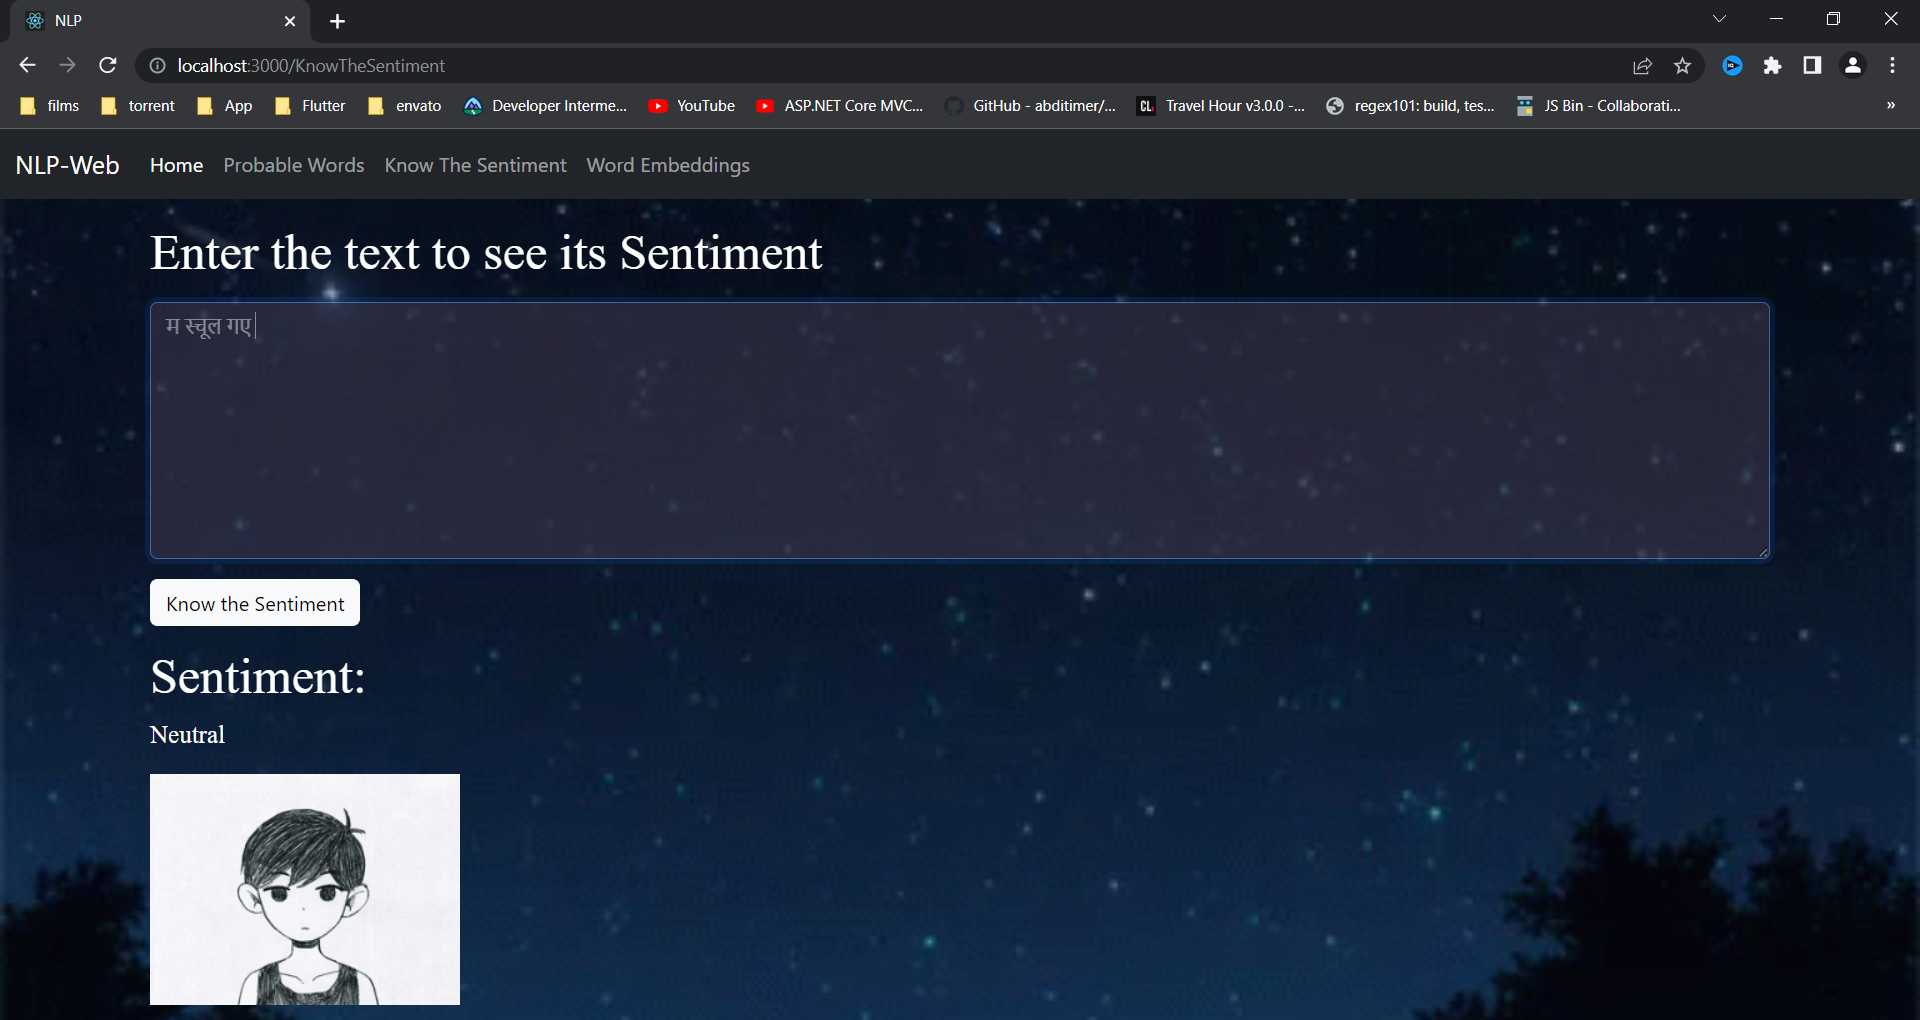
\includegraphics[scale = 0.2]{completed_task/frontend/sentiment_neutral.png}
	\caption{Sentiment classification (neutral) frontend}
	\label{fig:Sentiment classification (neutral) frontend}
\end{figure}

\begin{figure}[H]
	\centering
	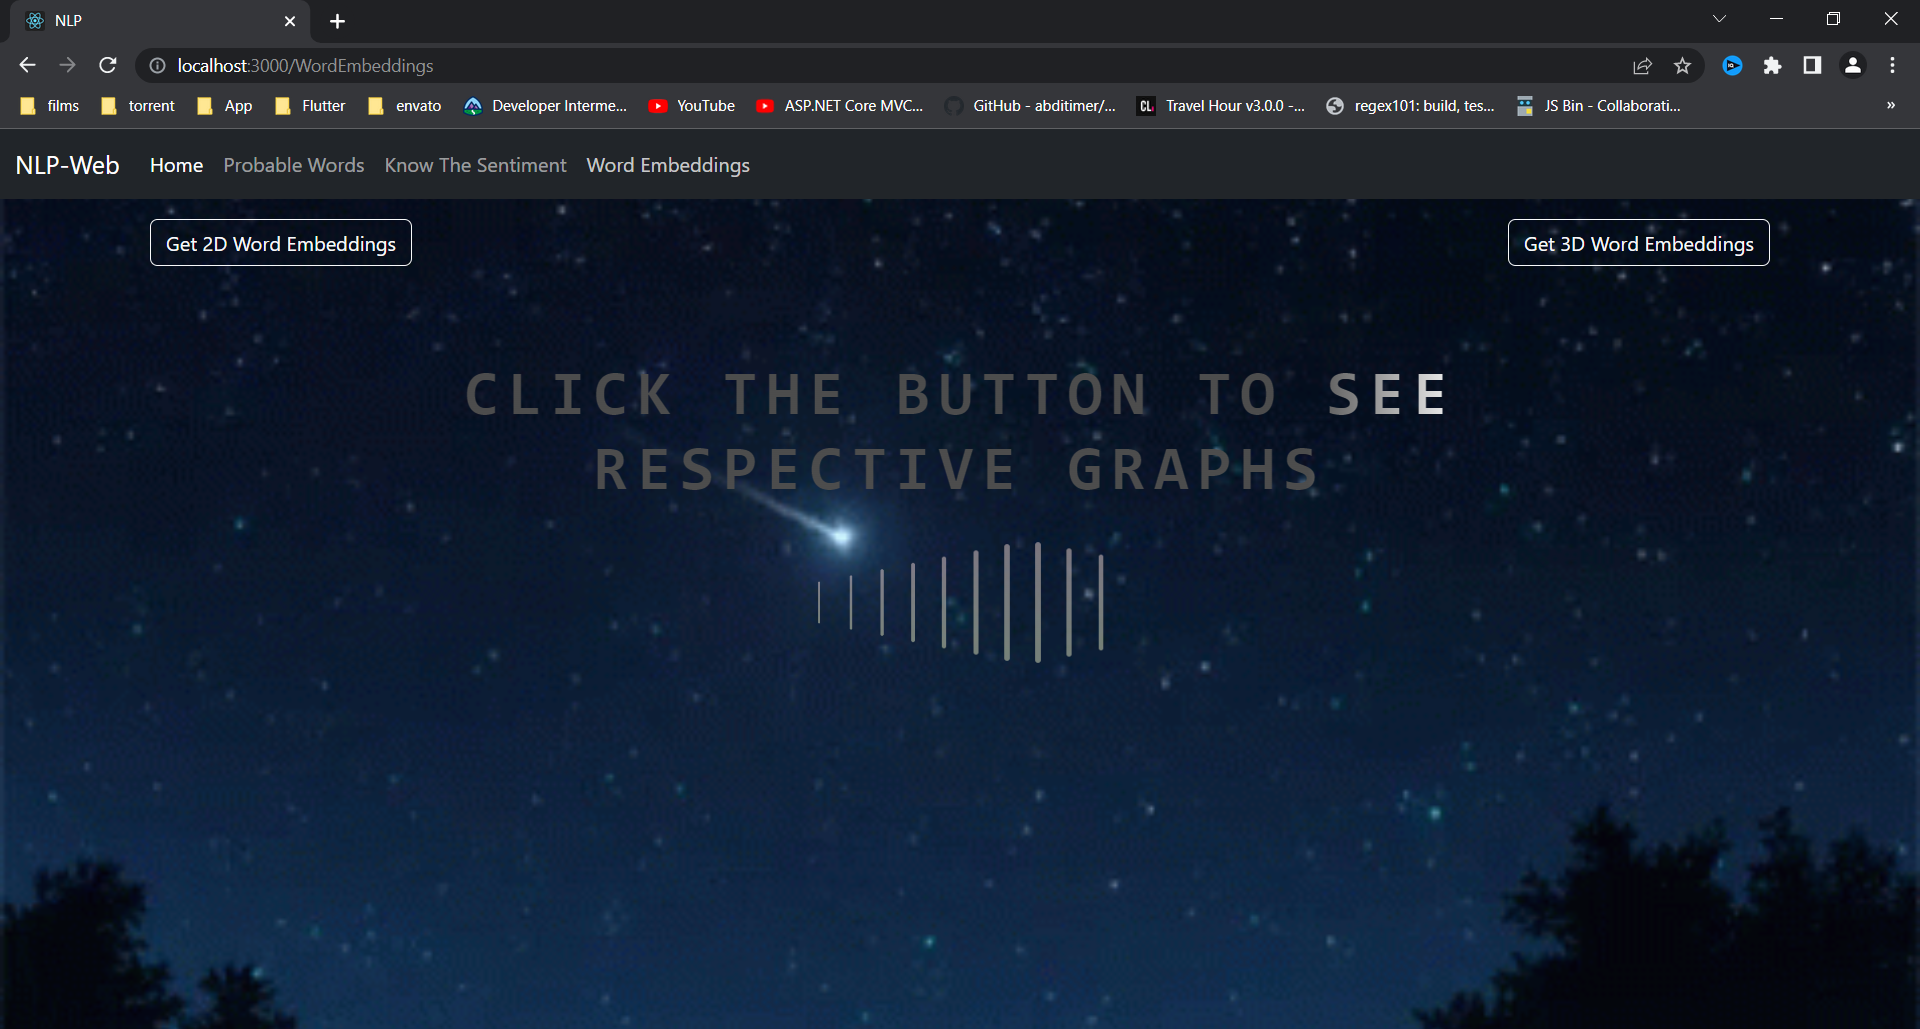
\includegraphics[scale = 0.2]{completed_task/frontend/word_embedding_front.png}
	\caption{Word Embedding frontend}
	\label{fig:Word Embedding frontend}
\end{figure}

\begin{figure}[H]
	\centering
	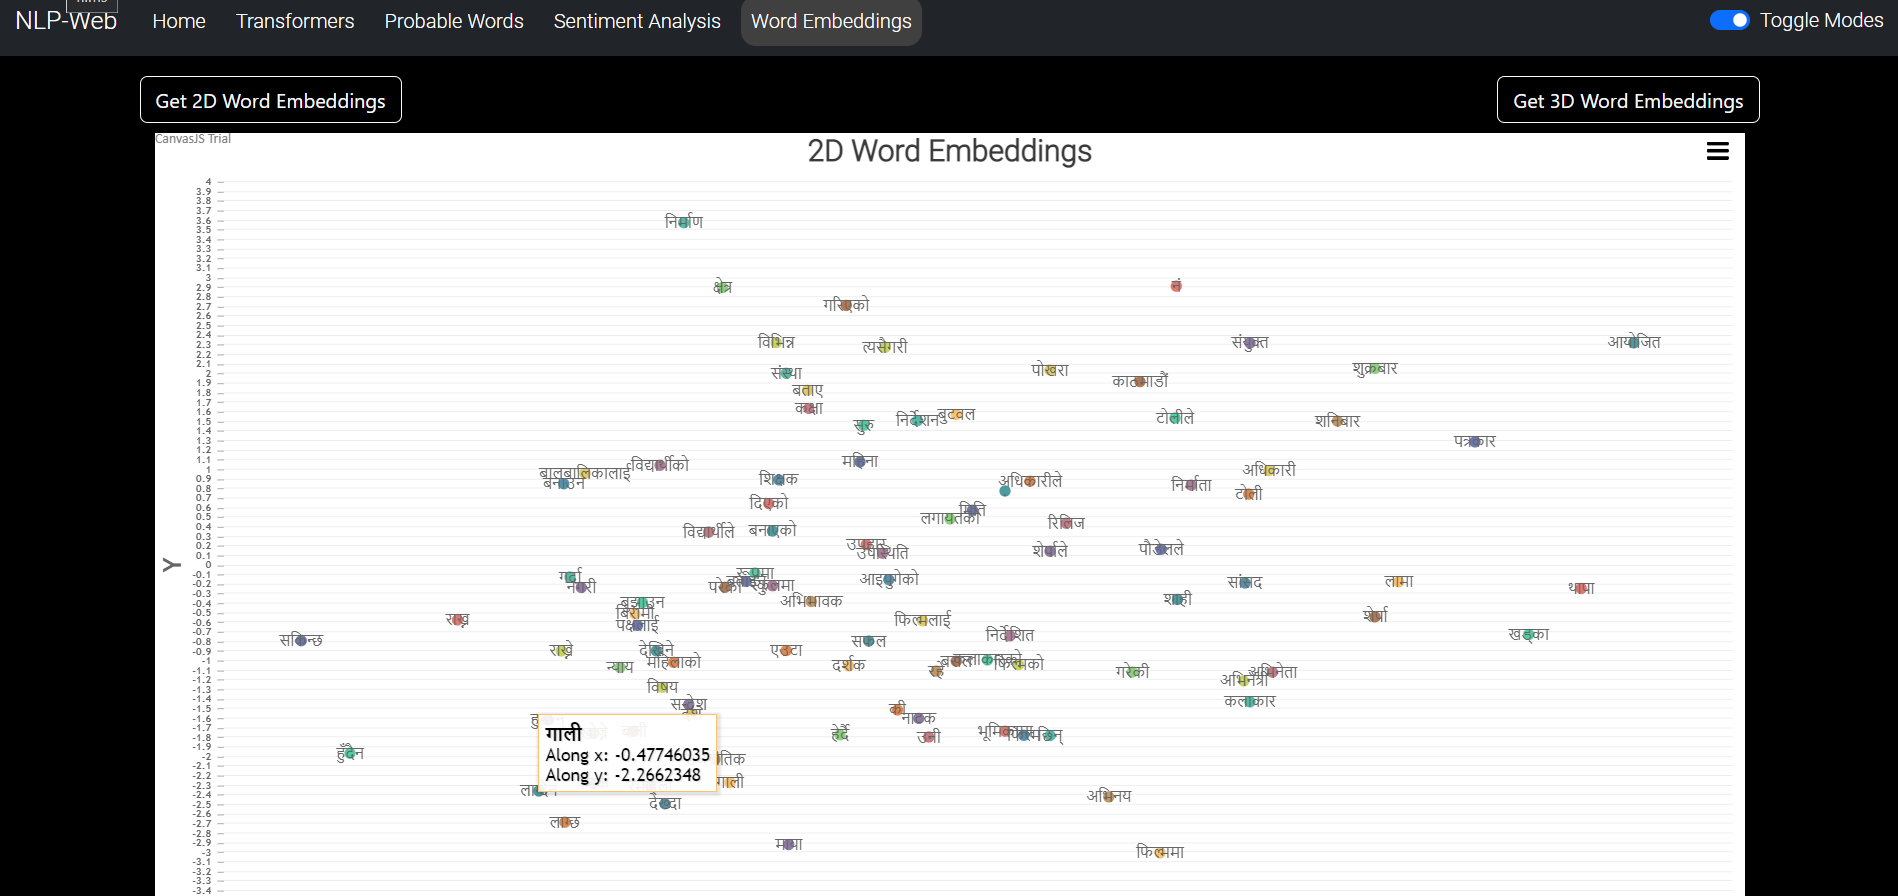
\includegraphics[scale = 0.2]{completed_task/frontend/word_embedding_2d.png}
	\caption{Word Embedding 2d plot frontend}
	\label{fig:Word Embedding 2d plot frontend}
\end{figure}




